\documentclass{article}
\usepackage{csquotes}
% Language setting
% Replace `english' with e.g. `spanish' to change the document language
\usepackage[backend=bibtex,bibencoding=ascii]{biblatex} %Imports biblatex package
\addbibresource{refs.bib}

\usepackage{enumitem}
\usepackage[english]{babel}
\usepackage{array}
\usepackage{amsmath}
\usepackage{pythonhighlight}
\usepackage{multirow}
\newcolumntype{P}[1]{>{\centering\arraybackslash}p{#1}}
\newcolumntype{M}[1]{>{\centering\arraybackslash}m{#1}}

% Set page size and margins
% Replace `letterpaper' with `a4paper' for UK/EU standard size
\usepackage[letterpaper,top=2cm,bottom=2cm,left=3cm,right=3cm,marginparwidth=1.75cm]{geometry}

\usepackage{amsmath}
\usepackage{graphicx}
\usepackage{caption}
\usepackage{subcaption}
\usepackage[colorlinks=true, allcolors=blue]{hyperref}
\usepackage{setspace}
\usepackage{booktabs}
\usepackage[T1]{fontenc}
\usepackage{longtable}
\doublespacing

\begin{document}
\newcommand{\Fig}[3]{\begin{figure}[!h!]\centering\includegraphics[width=0.5\linewidth]{#1}\caption{#2}\label{#3}\end{figure}}
\begin{titlepage}

\centering
\scshape


%
\rule{\textwidth}{1.6pt}\vspace*{-\baselineskip}\vspace*{2pt}
\rule{\textwidth}{0.4pt}

{\Huge \textbf{\textsc{ Fracture Mechanics and Impact \\
\vspace{15pt}}}}

\rule{\textwidth}{0.4pt}\vspace*{-\baselineskip}\vspace{3pt}
\rule{\textwidth}{1.6pt}\vspace{6pt}
\centerline{\textit{University of Illinois at Urbana-Champaign}} 
\centerline{\textit{Department of Nuclear, Plasma, and Radiological Engineering}}
\vspace{1.5\baselineskip}


\large \centerline{\textbf{Author:} Nathan Glaser}
\large \centerline{\textbf{Net-ID:} nglaser3}
\quad
\large \centerline{November 5, 2024}

\vfill{}

\includegraphics[width=0.8\textwidth]{./illinois.eps}\\[1cm]
%
\pagenumbering{gobble}
\end{titlepage}

\tableofcontents
\newpage
\pagenumbering{arabic}

\section{Abstract}

In this laboratory, we investigated the fracture mechanics and impact of PolyMethyl MethAcrylate (PMMA), High Density Poly-Ethylene (HDPE), 1045 Carbon Steel, 2024 and 7075 Aluminum Alloy. We set out to determine the critical fracture toughness, $K_{1C}$, of both aluminum alloys, and the impact energy absorbed and maximum load of PMMA, HDPE, 1045 Steel, and Aluminum 2024. Each of the 4 materials investigated through impact testing were conducted at 3 different temperatures, 0, 20, and 100 $^oC$, with the intent of gleaning a rough temperature dependence on the impact energy absorbed of each. We found $K_Q$ to be 35.36 $MPa\sqrt{m}$ and 30.44 $MPa\sqrt{m}$ for Aluminum 2024 and 7075, respectively. We determined the tests utilized to find these fracture toughness' to be valid, meeting all pre-defined criteria. We found a strong correlation between temperature and impact energy for HDPE, PMMA, and 1045 Steel, but not for 2024 Aluminum. We determined the lac of a relation to be due to the transitional temperature for Aluminum 2024 to be much higher than the range of temperatures we tested. Finally, we found the maximum load applied during an impact test to be a poor predictor of impact energy absorbed, and thus fracture toughness. We found potential sources of error to reside predominantly in the uncertainty of the temperature of each specimen during testing. 

\section{Introduction}

This laboratory aimed to investigate the fracture mechanisms of various aluminum / steel alloys and plastic polymers. The fracture mechanisms of materials are exceedingly important material properties to have a grasp on. Most important among these properties is the fracture toughness. Fracture toughness can hold the form of three different properties, but all mean similair things. The fracture toughness is defined as the resistance of a material to crack propagation under load. Essentially, this is a measure of how resistive a material is to a crack growing while the material has external forces enacted upon it. 

The derivation of the fracture toughness properties is strenuous and long-winded, and thus the reader will be spared. If desired, a complete derivation of the fracture toughness can be found in \cite{manual}. While the full derivation is long, a description of the result is easily digestible, adn hence presented. The critical fracture toughness, $K_{1C}$, is defined as:

\begin{equation}
    K_{1C} = \sigma_{nom}\sqrt{\pi a_{cr}}
\end{equation}

$K_{1C}$ is a material property that is tested for, however once this value is found an accurate estimate of the nominal critical stress required to induce fracture given a crack of length $2a$. This is extremely important, as one may not know the exact load applied to a material, but can easily determine whether this load is near critical failure.

Proximally, fracture mechanics vary depending on temperature. This is tested through impact testing. Unfortunately, $K_{1C}$ cannot be directly tested for with impact testing, but an analogous quantity can be ---- energy absorbed before fracture. The higher amount of energy a material absorbs prior to catastrophic fracture can be seen as a higher resistance to fracture, especially given impact test specimens have pre-inscribed notches to simulate a crack. Importantly, when investigating specimens impact energy absorbed as a function of temperature, there will be a sudden sharp change in the quantity observed. This is due to temperature induced phase change within the material. For 1045 Steel and 2024 Aluminum this hold ths form of converting from Face Centered Cubic (FCC) to Body Centered Cubic (BCC), presented in Fig. \ref{fig:bccfcc}. In plastic polymers this is dubbed as the 'glass transtion'.

\begin{figure}[!h!]
    \centering
    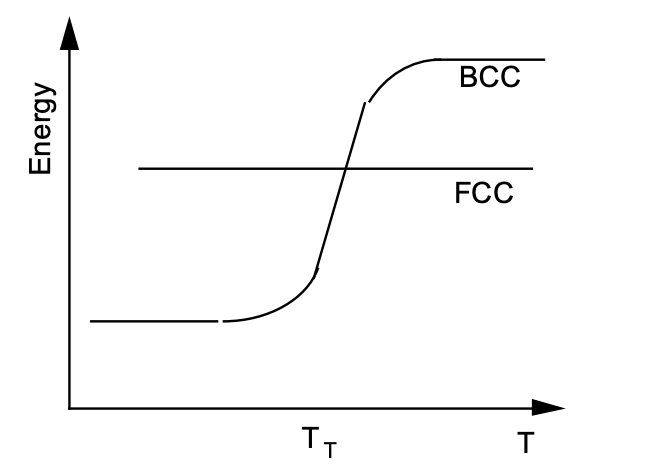
\includegraphics[width=0.5\linewidth]{plots/bccfcc.png}
    \caption{Temperature induced transition from FCC to BCC}
    \label{fig:bccfcc}
\end{figure}

\section{Experimental Methods}
We conducted two distinct experiments in this laboratory. The first was Impact testing, and the second was Compact Tension testing. The experimental procedures we undertook were adopted from \cite{manual}. 

First, the following are the procedures we undertook for the impact testing:
\begin{enumerate}
    \item With an optical microscope we measured the notch radius of the charpy specimens
    \item With a caliper, we measured the length, height, and width of each specimen, as well as notch depth
    \item After measuring the dimensions of each specimen, we then subjugated it to a prescribed temperature: $0 ^oC$, $20 ^oC$, or $100 ^oC$
    \item Once the specimen was at the desired temperature, it was quickly loaded into the vertical drop impact test machine, and the impacter was then dropped. The speed of loading was crucial to maintain the intended temperature
    \item After impact, the machine was returned to its starting point, and we investigated the specimen to determine the type of fracture it experienced
\end{enumerate}

Second, the following are the procedures we undertook for the compact tension testing: 

\begin{enumerate}
    \item Measured the diameter of the circular grips, the distance from the circular grips to each side, the full width, and the depth of the pre-crack, as well as the overall thickness of the specimen
    \item with all of the aforementioned measurements, we determined $a_0$ the distance from the center-of-loading to the point of the crack, and $W$, the distance from the center-of-loading to the edge of the specimen
    \item We loaded the specimen into the compact tension tester, then put the specimen under tension until failure
\end{enumerate}

Further, Each specimen utilized in the compact tension testing had undergone pre-test loading. We did not conduct this as this takes much longer time than we have in laboratory. The pre-test loading parameters for each specimen are:

\begin{table}[!h!]
    \centering
    \caption{Pre-load parameters for Aluminum Alloys 7075 and 2024 }
    \begin{tabular}{|c|c|c|c|c|}
        \midrule
        \bottomrule
         Material & $P_{low}$  [kN] & $P_{high}$  [kN]& Frequency  [Hz] & Number of Cycles \\
         \toprule
         \bottomrule
         Aluminum 7075 & 0.5 & 8.0 & 4.0 & 18,000 \\
         \hline
         Aluminum 2024 & 1.0 & 10.0 & 4.0 & 16,000 \\
         \hline
    \end{tabular}
    \label{tab:preloadParams}
\end{table}

\section{Theoretical Models}
To begin, the experiments carried out in this lab were two-fold: Impact testing and Compact Tension testing. We predominantly utilized theoretical models in specifically fracture toughness investigation of the compact tension test results. 

To begin, the stress intensity factor ($K_1$) for the compact specimen follows:
\begin{equation}
    K_{1} =  \frac{P}{t\sqrt{W}}f\left( \frac{a}{W}\right)
    \label{eq:k1c}
\end{equation}

where $f\left( \frac{a}{W}\right)$ is a geometric correct factor. For the geometry of the specimen we utilized, the accepted ASTM correlation is \cite{manual}:

\begin{equation}
    f\left(\frac{a}{W}\right) = .886+4.64\left(\frac{a}{W}\right) −13.32\left(\frac{a}{W}\right)^2+14.72\left(\frac{a}{W}\right)^3−5.6\left(\frac{a}{W}\right)^4
\end{equation}

When actually performing the experiment, there are three potential outcomes (assuming the test is valid). These three outcomes are presented below, in Fig. \ref{fig:3types}. Type I results from a specimen that experiences  plastic deformation at the crack-tip, with relatively constant size. Type II results from a specimen that experienced a crack that grew in size, but then suddenly stopped growing, and then failed after further loading. 

\begin{figure}[!h]
    \centering
    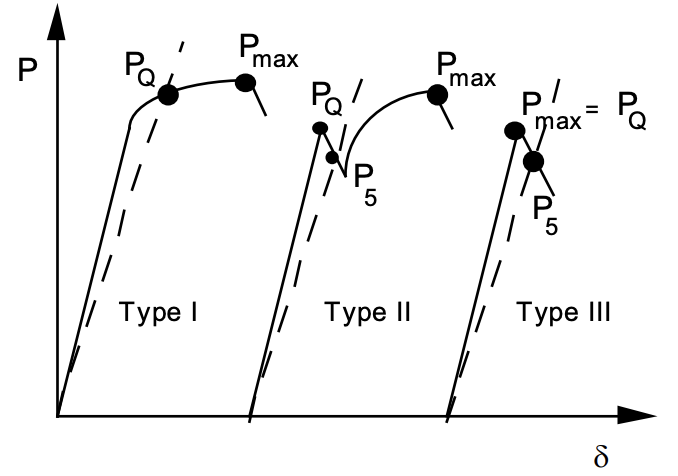
\includegraphics[width=0.5\linewidth]{plots/3types.png}
    \caption{Three types of load-displacement curves}
    \label{fig:3types}
\end{figure}

For Type I and II curves, the P utilized in \eqref{eq:k1c} is found by finding the intercept of the $95\%$ secant line with the curve and by finding the maximum load prior to the intercept of the secant line with the curve, respectively. For Type III this P is simply the maximum load applied to the specimen. 

Finally, after selecting the most apt generalized curve and finding the resulting $K_Q$ value, the validity of the test must be investigated to say whether $K_Q$ is equal to $K_{1C}$. A test must pass all of the following criteria for it to be deemed valid:

\begin{enumerate}
\label{enum:constraints}
    \item $P_{precrack} < 0.6 P_Q$
    \item $P_{max} < 1.1 P_Q$
    \item a and W must both be $> 2.5 \left(\frac{K_Q}{\sigma_{ys}}\right)^2$
    \item $0.45 < \frac{a}{w} < 0.55$
\end{enumerate}
\newpage
\section{Results}
To begin, we found the impact energy absorbed by each specimen as a function of energy for both sets of data. The data collected by groups A and B are presented on the left, and the data collected by groups C and D are presented on the right. The resulting figures are shown in Fig. \ref{fig:q1e}. Further, we found the maximum applied load to each specimen as a function of energy. Again, the data collected by groups A and B are presented on the left, and the data collected by groups C and D are presented on the right. The resulting figures are shown in Fig. \ref{fig:q1l}.

\begin{figure}[!h!]
    \centering
    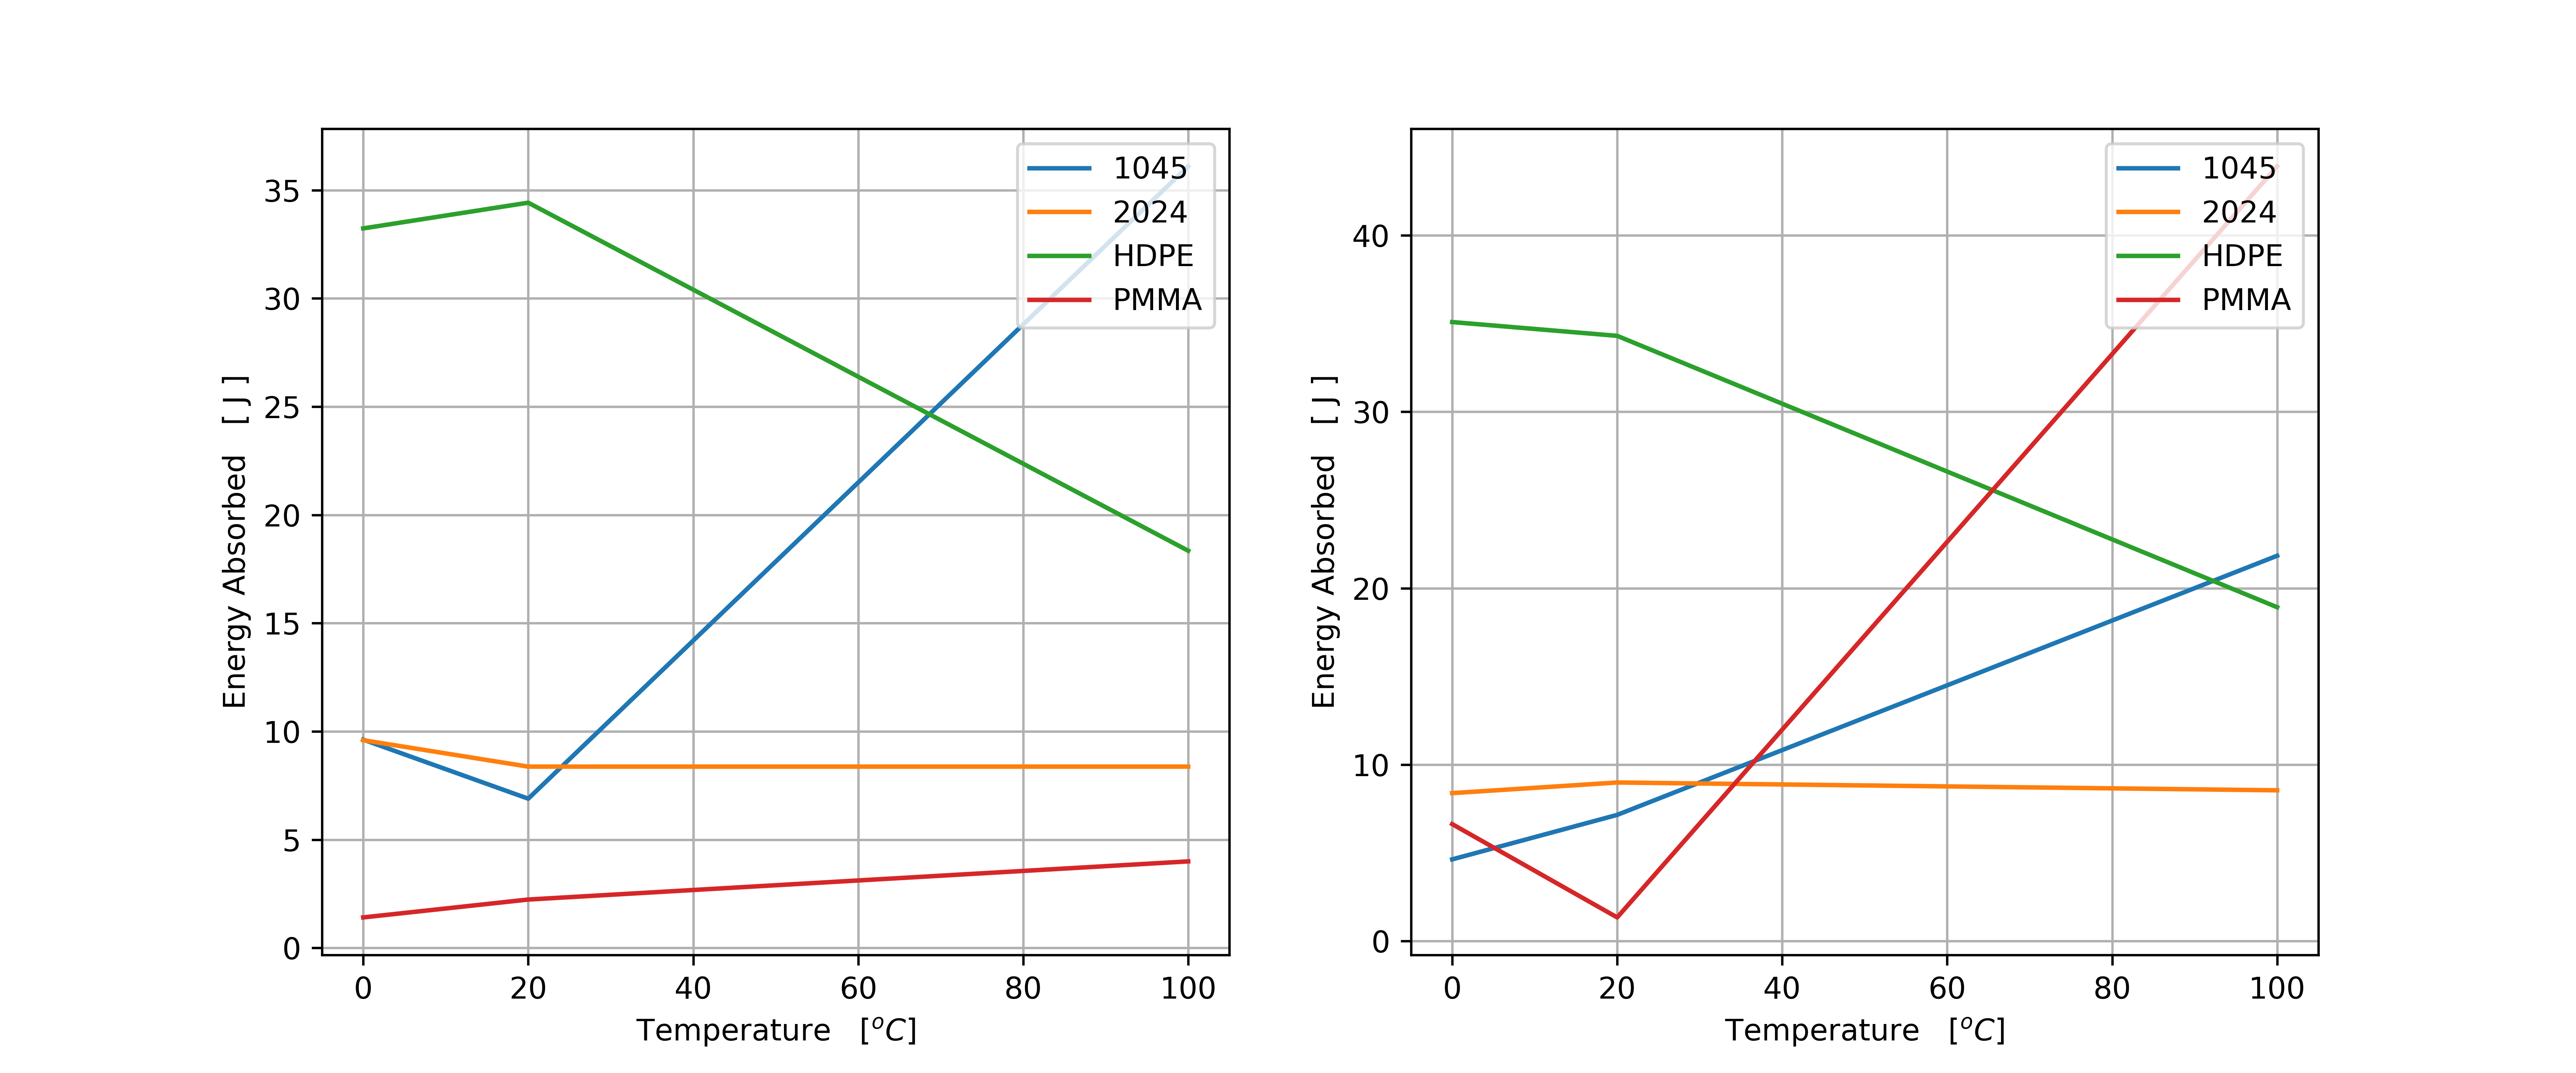
\includegraphics[width=\linewidth]{plots/q1_energy.png}
    \caption{Impact energy absorbed as a function of temperature for each material}
    \label{fig:q1e}
\end{figure}

\begin{figure}[!h!]
    \centering
    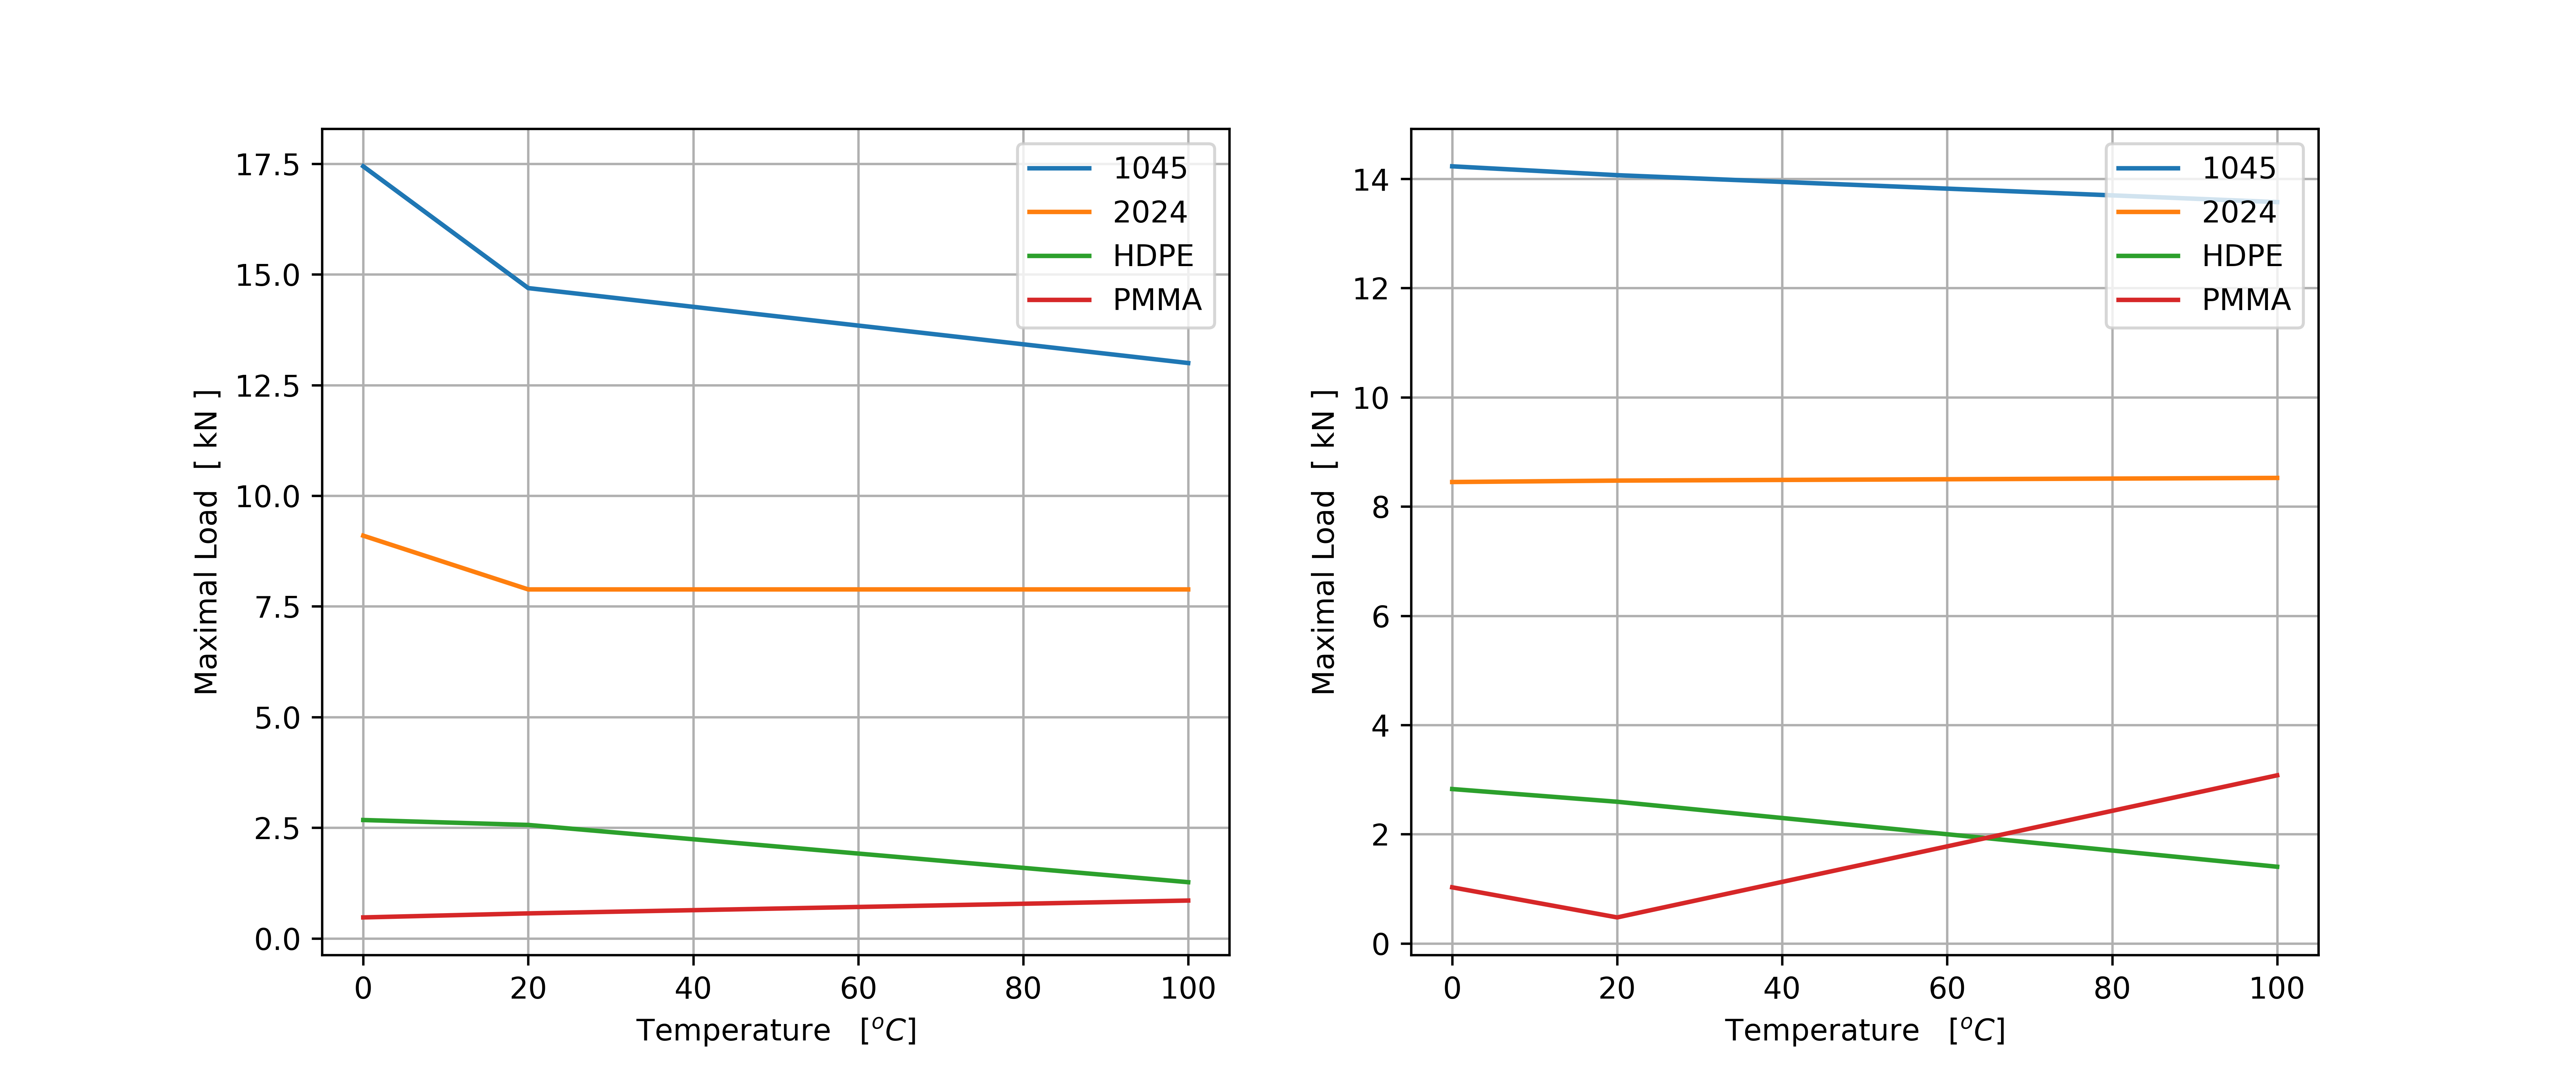
\includegraphics[width=\linewidth]{plots/q1_load.png}
    \caption{Maximum applied Load as a function of temperature for each material}
    \label{fig:q1l}
\end{figure}

\newpage
To continue, we found the energy absorbed, the maximum applied load, time to failure, and type of fracture for each tested specimen. This data is presented in Tab. \ref{tab:q2}. 

\begin{table}[!h!]
    \centering
    \caption{Select Experimental Results for Each Specimen }
    \renewcommand{\arraystretch}{1.5}
    \begin{tabular}{|c|c|c|c|c|}
        \toprule
        \hline
        Specimen & Energy Absorbed [J]& Maximum Load [N]& Time to Failure [s]& Fracture Type\\
        \toprule

        \bottomrule
        \multicolumn{5}{|c|}{Groups A and B} \\
        \toprule
        \bottomrule
        1045 at 0C & 9.619 & 17441.723 & 1.026 & Brittle\\ 
        \hline
        1045 at RT & 6.892 & 14690.818 & 0.458 & Brittle\\ 
        \hline
        1045 at BW & 36.104 & 12997.954 & 2.064 & Ductile\\ 
        \hline
        2024 at 0C & 9.594 & 9097.932 & 0.850 & Brittle \\ 
        \hline
        2024 at RT & 8.373 & 7883.913 & 0.852 & Brittle\\ 
        \hline
        HDPE at 0C & 33.236 & 2674.698 & 6.860 & Ductile \\ 
        \hline
        HDPE at RT & 34.424 & 2563.510 & 7.360 & Ductile\\ 
        \hline
        HDPE at BW & 18.346 & 1270.430 & 7.700 & Brittle \\ 
        \hline
        PMMA at 0C & 1.407 & 474.392 & 6.76 & Brittle\\ 
        \hline
        PMMA at RT & 2.233 & 565.541 & 7.0 & Brittle \\ 
        \hline
        PMMA at BW & 3.995 & 855.563 & 8.04 & Brittle\\ 
        \toprule
        
        \bottomrule
        \multicolumn{5}{|c|}{Groups C and D} \\
        \toprule
        \bottomrule
        1045 at 0C & 4.627 & 14229.919 & 0.178 & Brittle\\ 
        \hline
        1045 at RT & 7.149 & 14067.589 & 0.236 & Brittle \\ 
        \hline
        1045 at BW & 21.841 & 13574.803 & 1.062 & Mixed / Ductile\\ 
        \hline
        2024 at 0C & 8.383 & 8449.110 & 0.856 & Brittle\\ 
        \hline
        2024 at RT & 8.985 & 8475.063 & 0.882 & Brittle\\ 
        \hline
        2024 at BW & 8.543 & 8524.085 & 0.86 & Brittle\\ 
        \hline
        HDPE at 0C & 35.091 & 2827.067 & 10.3 & Ductile \\ 
        \hline
        HDPE at RT & 34.309 & 2594.395 & 10.64 & Ductile\\ 
        \hline
        HDPE at BW & 18.923 & 1404.268 & 10.6 & Ductile \\ 
        \hline
        PMMA at 0C & 6.627 & 1027.504 & 8.24 & Brittle\\ 
        \hline
        PMMA at RT & 1.336 & 476.463 & 6.78 & Brittle\\ 
        \hline
        PMMA at BW & 43.921 & 3078.368 & 13.16 & Ductile\\ 
        \toprule
    \end{tabular}
    \label{tab:q2}
\end{table}

\newpage

Next, we found the the applied load as a function of displacement for Aluminum 2024 and Aluminum 7075. These are presented in Fig. \ref{fig:q4}. Tangentially, we found the associated $P_Q$ and $P_{max}$ of both of the aforementioned Aluminum alloys. For the Aluminum 2024 alloy, we determined the most apt description of the plot was a Type I plot, and thus we utilized a $95\%$ secant line to determine $P_Q$. For Aluminum 7075, we determined type III plot to be the most apt description, and thus $P_Q$ is equal to $P_{max}$. These values are tabulated in Tab. \ref{tab:q4}.

\begin{figure}[!h!]
    \centering
    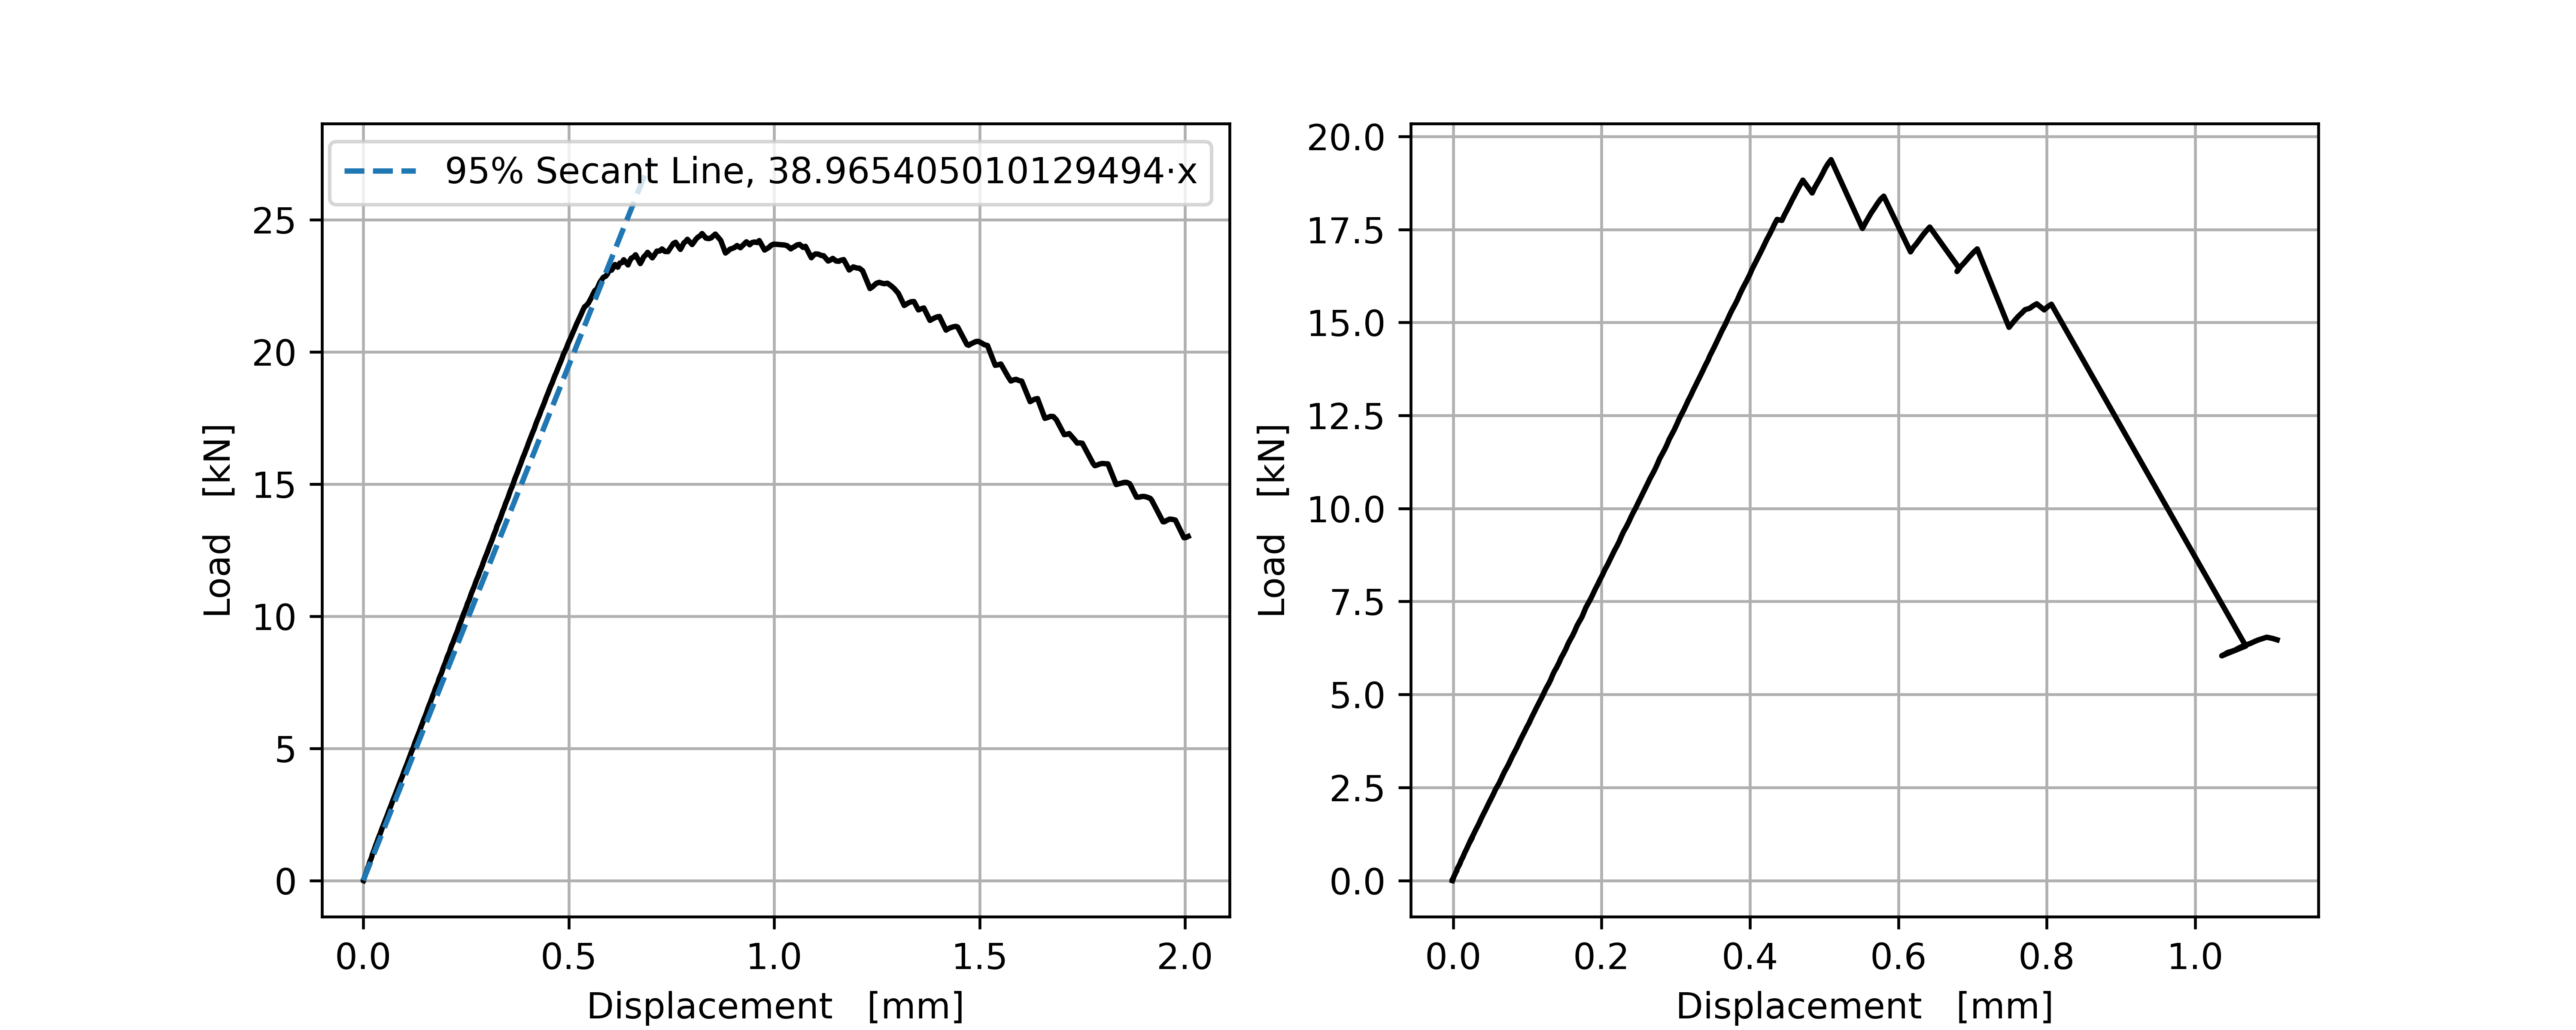
\includegraphics[width=\linewidth]{Lab6/plots/q4.png}
    \caption{Load against displacement for Aluminum 2024 and 7075, respectively}
    \label{fig:q4}
\end{figure}

\begin{table}[!h!]
    \centering
    \caption{$P_Q$ and $P_{max}$ for Aluminum alloys 2024 and 7075}
    \begin{tabular}{|c|c|c|}
         \toprule
         \hline
         Material & $P_Q$ & $P_{max}$ \\
         \toprule
         \bottomrule
         Al. 2024 & 22.836 & 24.479 \\ 
         \hline
         Al. 7075 & 19.376 & 19.376 \\
         \hline
    \end{tabular}

    \label{tab:q4}
\end{table}

From these $P_Q$ values, we determined $K_Q$ to be 35.36 $MPa\sqrt{m}$ and 30.44 $MPa\sqrt{m}$ for Aluminum 2024 and 7075, respectively.

\newpage
\section{Analysis and Discussion of Results}

In this section we will examine potential sources of error. First, and most notably, the specimens used in impact testing were likely not at the prescribed temperatures. This source of this error is twofold. The first is that specimens were not allowed to reach their designated temperatures, and second is that the specimens were likely left in ambient conditions after their respective temperature acclimation phases, resulting in a net return to ambient temperatures. This is a very strong source of error most notably seen in the PMMA trials. PMMA has a transition temperature at around 100 $^oC$, and thus will react very differently depending on the precise temperature of the specimen ---- 98$^oC$ will behave very differently than 100 $^oC$. A further source of error is the lack of a room temperature specimen for Aluminum 2024 by groups A and B, resulting in lower statistics to compare and glean meaningful results from. 


\section{Answers to Questions}

To begin, we found the impact energy absorbed by each specimen and the maximum load applied to each specimen throughout the impact testing. The restuls of these are plotted as a function of temperature in Figs. \ref{fig:q1e} and \ref{fig:q1l}, respectively.

Next, we determined the impact energy absorbed, the maximum load, the time to failurem and the fracture type of each specimen, presented in Tab. \ref{tab:q2}. We can determine the ductility of each material through investigation of the energy absorbed by the material. The higher the energy absorbed, the more ductile a material is. This stems from one of the definitions of ductility, derived from toughness, or energy absorbed. Thus, HPGE is extremely ductile at all temperatures, where Aluminum alloy 2024 is in a mixed region. Further, Steel 1045 acts more as a mixed material at low temperatures, but at high relative temperatures becomes ductile. This is expected as there is a transition temperature roughly between 20 $^oC$ and 100 $^oC$. Finally, PMMA is an odd-case. PMMA is a very brittle material at low temperatures, but has a transition temperature very close to 100 $^oC$. This transition temperature being very close to the temperature we were measuring at resulted in two very different data points. PMMA after reaching this transition temperature is extremely ductile. The quantities of maximum load and energy absorbed are not solely functions of each other, but are very clearly related. Keeping the time to failure constant across trials, or normalizing by the time to failure, there appears to be a roughly linear trend. As the maximal load increases, so does the energy absorbed. This makes inherit sense as the more force applied to an object prior to fracture, the more energy the object must absorb to not fracture. However, due to the dependence of energy absorbed on both maximum load and time to failure, we can not responsibly characterize the toughness of a material with only measuring the maximum load. A clear example of this is Group A and B's 1045 trials. Only investigating the maximum load would insinuate lower toughness, but this is the opposite of reaility. The disparity comes from the time to failure of the specimens.

From Figs. \ref{fig:q1e} and\ref{fig:q1l}, we can determine which materials have a transitional temperature in the domain of temperatures we tested. Without a doubt, HDPE and Steel 1045 have transitionary temperatures. These transition temperatures are roughly at  50 $^oC$ and 40 $^oC$, respectively. PMMA also has an transition temperature, as evident in the second data-set. This temperature must be very close to, if not, 100 $^oC$ for the results at 100 $^oC$ to be so starkly different between the two data-sets. We would expect to see a more obvious trend in PMMA at 100 $^oC$ if we tested higher temperatures, and we expect Aluminum 2024 to have a transitional temperature past 100 $^oC$. In contrast to our approximated results, we find the transition temperatures of PMMA, Steel 1045, and HDPE to be 105 $^oC$ \cite{pmma}, 25 $^oC$ \cite{1045}, and 42 $^oC$ (assuming 15\% glass bead content) \cite{hdpe}.

Finally, to determine the $K_{1C}$ values for aluminum 2024 and 7075, we first found the load-displacement curves, and the resulting $P_Q$ values. These curves are presented in Fig. \ref{fig:q4}, and the $P_Q$ values are presented in Tab. \ref{tab:q4}. We found the Aluminum 2024 curve to be type I, and the Aluminum 7075 curve to be type III. For Aluminum 2024 we found $K_{1C}$ to be 35.36 $MPa\sqrt{m}$, and for Aluminum 7075 we found $K_{1C}$ to be 30.44 $MPa\sqrt{m}$. To investigate the validity of these results we will differ back to the constraints presented in Enum. \ref{enum:constraints}. For both trials $P_{max} < 1.1 P_Q$, and $P_{pre-crack} < 0.6 P_Q$. For Aluminum 2024 and 7075, the $\frac{a}{w}$ ratio
was 0.471 and 0.475, respectively. Thus our test results are valid. 
\section{Conclusions}
To conclude, we de determined a strong correlation between temperature and impact energy absorbed for three of the four materials tested. These three materials (HDPE, PMMA, and 1045 Steel) had this temperature dependence due to the presence of a transitional temperature residing within the domain of the temperatures we tested. For HDPE and PMMA this is known as the glass transitional temperature, and for the 1045 steel this is the transitional temperature from FCC to BCC. We found no convincing correlation between temperature and impact energy for 2024 Aluminum, likely due to the lack of a transitional temperature between 0 and 100 $^oC$. Further, we found no convincing correlation between maximum load applied during an impact test and impact energy absorbed by the specimen. We determine that while the impact energy is a function of maximum load, it is not linear and depends more on \textit{sustained load} than peak load. This inherently makes sense as a the energy absorbed by the material prior to fracture, the toughness, is the integral under the stress strain curve. Thus, the peak load may matter, but if a smaller load is sustained for much much longer the energy absorbed will be higher for the smaller load. Finally, we found $K_Q$ to be 35.36 $MPa\sqrt{m}$ and 30.44 $MPa\sqrt{m}$ for Aluminum 2024 and 7075, respectively. We determined the tests utilized to find these fracture toughness' to be valid, meeting all pre-defined criteria. While the criteria $\frac{a}{W}$ was on the lower side for both trials, they were both well within the criteria bounds. 
\section{References}

\printbibliography[heading=none]
\end{document}